\section{Multi-objective Weight Optimization}

With an accurate CPU model, the weights must now be tuned to match measured
power consumption on real hardware. We formulate this as a multi-objective
optimization problem.

We start by creating a set of training workloads, essentially computer programs
designed to hold certain characteristics compiled to a native
ARMv7\footnote{ARMv7 is the instruction set supported by ARM Cortex-A9.} binary.
The design and selection of these will be elaborated in the next section. We
execute the binaries in the gem5 simulator with the CPU model from last
section to obtain a file containing \texttt{(time, event)} tuples from the
(modelled) execution, just like in \autoref{lst:trace}. The next challenge is to
assign each of these events a cost.

We attack this problem by running a multi-objective optimization algorithm. We
pick a subset of event types that is believed to impact energy consumption, as
we described in \autoref{subsec:powerevents}. Choosing too many events could
give us overfitting issues, but taking too few out could lead to lack of detail
in our model. We experimented with dozens of optimization algorithms and ended
up combining a $1 + \lambda$ evolutionary strategy with simulated annealing. The
evolutionary part would make sure that our algorithm was explorative enough
(i.e. it covered large parts of the solution space), while the simulated
annealing part made the algorithm more aggressive to start with.  Using DEAP
\cite{DEAP_JMLR2012}, a Python framework for evolutionary algorithms, we were
able to prototype our ideas rapidly. The pseudocode in
\autoref{lst:ga-algorithm} describes the algorithm we ended up on.

\begin{lstlisting}[caption={Algorithm used to evolve a set of event weights},label={lst:ga-algorithm}]
Generate 10 random individuals
%TODO: Insert rest of algorithm here
\end{lstlisting}

\begin{figure}
    \centering
    \def\svgwidth{\columnwidth}
    \includegraphics[width=\textwidth]{figs/ga_genome.pdf}
\end{figure}

The genome is a set of CPU events, each mapped to an energy cost. E.g.
\texttt{\{IntAlu: 170, IntMult: 1300, MemRead: 80, MemWrite: 50, SimdFloatMisc:
1400, L1R: 230, L1W: 340, L2R: 1100, L2W: 1300, PhysR: 2600, PhysW: 2800\}} is a
valid individual in the population. To calculate the fitness of an individual,
we run PET with the genome weights on a set of workloads and compare the energy
profiles with measurements on hardware.

We emphasize that the use of an evolutionary algorithm is an arbitrary choice;
technically, we could have picked any algorithm to do this for us. When the
weights have evolved to match our hardware measurements, we no longer care how
these weights were obtained.
